\newpage
\section{Auswertung}
\label{sec:Auswertung}
\subsection{Fehlerrechnung}
Für die Fehlerrechnung wird die Gaußsche Fehlerfortplanzung
\begin{equation}
\Delta f=\sqrt{\left(\frac{\partial f}{\partial x}\right)^2(\Delta x)^2+\left(\frac{\partial f}{\partial y}\right)^2(\Delta y)^2+...+\left(\frac{\partial f}{\partial z}\right)^2(\Delta z)^2}
\end{equation}
für fehlerbehaftete Werte $x,y,...,z$ mit den Unsicherheiten $\Delta x,\Delta y,..,\Delta z$ sowie der Fehler des Mittelwertes $\bar{x}$:
\begin{equation}
\Delta \bar{x}=\sqrt{\frac{1}{N(N-1)}\sum_{k=1}^N(x_k-\bar{x})^2}
\end{equation}
verwendet.
\subsection{Invertierender Verstärker}
Für den invertierenden Verstärker wurden die Amplitude und die Phasenverschiebung $\Phi$ der Amplitude der Ausgangsspannung $U_A$ in Abhängigkeit von der Frequenz $f$ gemessen. Eine solche Messung wurde mit drei verschiedenen Konfigurationen von Wiederständen ausgeführt.

Mittels der Eingangsamplitude des Signalgenerators wurde für alle Messungen aus den gemessenen Amplituden jeweils die Verstärkung $G$ bestimmt und anschließend in einem doppellogarithmischen Koordinatensystem in Abhängigkeit von der Frequenz abgebildet.
\begin{figure}
\centering
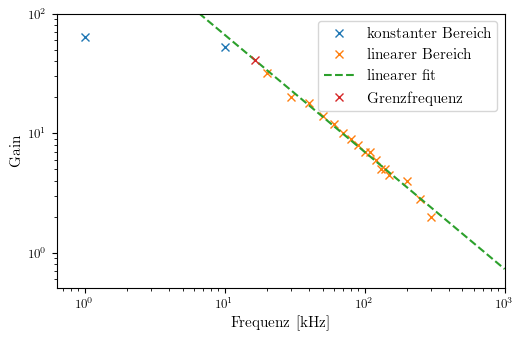
\includegraphics[width=0.6\textwidth]{Frequenzgang Messreihe1}
\caption{Verstärkung in Abhängigkeit von der Frequenz in doppellogarithmischer Darstellung für einen invertierenden Verstärker mit Wiederständen $R_1=\SI{1}{\kilo\ohm}$ und $R_2=\SI{68}{\kilo\ohm}$}
\label{fig:invert_freq_1}
\end{figure}

\begin{figure}
\centering
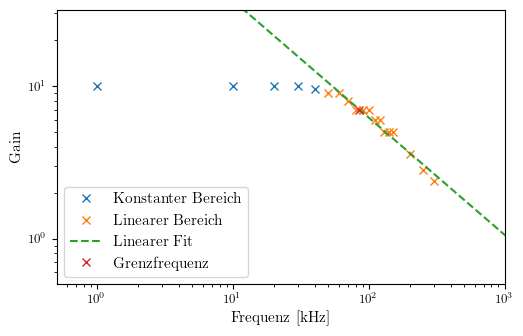
\includegraphics[width=0.6\textwidth]{Frequenzgang Messreihe2}
\caption{Verstärkung in Abhängigkeit von der Frequenz in doppellogarithmischer Darstellung für einen invertierenden Verstärker mit Wiederständen $R_1=\SI{10}{\kilo\ohm}$ und $R_2=\SI{100}{\kilo\ohm}$}
\label{fig:invert_freq_2}
\end{figure}

\begin{figure}
\centering
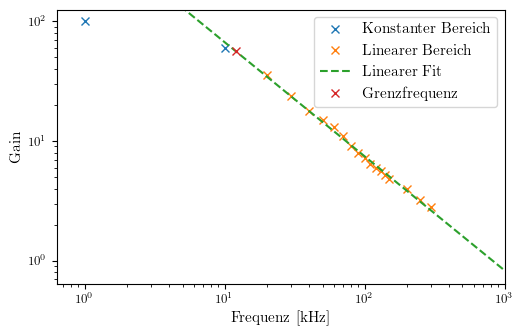
\includegraphics[width=0.6\textwidth]{Frequenzgang Messreihe3}
\caption{Verstärkung in Abhängigkeit von der Frequenz in doppellogarithmischer Darstellung für einen invertierenden Verstärker mit Wiederständen $R_1=\SI{1}{\kilo\ohm}$ und $R_2=\SI{100}{\kilo\ohm}$}
\label{fig:invert_freq_3}
\end{figure}

\begin{figure}
\centering
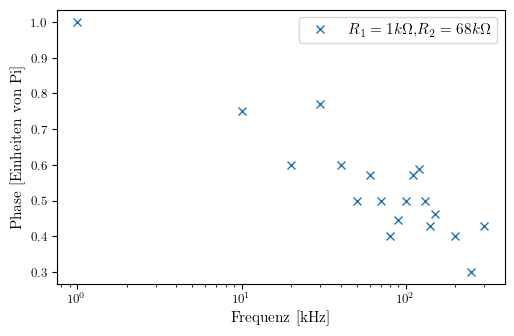
\includegraphics[width=0.6\textwidth]{Operationsverstärker Phase1}
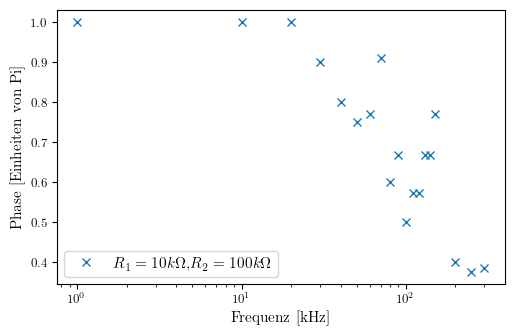
\includegraphics[width=0.6\textwidth]{Operationsverstärker Phase2}
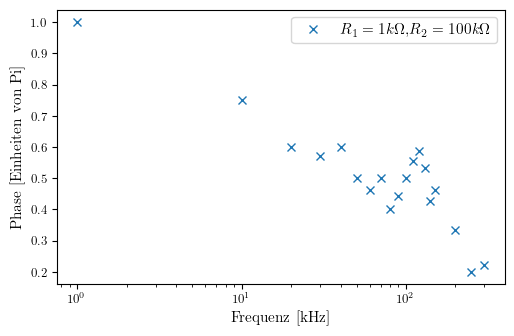
\includegraphics[width=0.6\textwidth]{Operationsverstärker Phase3}
\caption{Phasenverschiebung in Einheiten von $\pi$ abhängig von der Frequenz in halblogarithmischer Darstellung für einen invertierenden Verstärker für alle die drei vorgenommenen Messreihen}
\label{fig:invert_freq_Ph}
\end{figure}
Die Ergebnisse sind in den Abbildungen \ref{fig:invert_freq_1}, $\ref{fig:invert_freq_2}$, $\ref{fig:invert_freq_3}$ dargestellt. Die Phasenverschiebungen der drei Messreihen finden sich in Abbildung $\ref{fig:invert_freq_Ph}$.
Im Bereich des linearen Zusammenhangs zwischen beiden Größen kann ein Fit der Form:
\begin{equation}
\log(G)=m\log(f)+b
\end{equation}
welche im nicht logarithmischen Raum einer Funktion der Form:
\begin{equation}
G(f)=Bf^m
\end{equation}
entspricht. Für die drei Messreihen lauten die Fitfunktionen:
\begin{gather}
G_1(f)=(634,79\pm76,14)f^{-0,98\pm0,26} \\
G_2(f)=(157,25\pm36,32)f^{-0,71\pm0,05} \\
G_3(f)=(605.03\pm63,597)f^{-0,95\pm0,02}
\end{gather}
Die annähernd konstante Verstärkung im niederfrequenteren Bereich $G_c$ kann durch den Mittelwert der entsprechenden Messpunkte ermittelt werden. Mithilfe dieses Wertes sowie der gefitteten Funktionen im linearen Bereich kann die Grenzfrequenz $f_g$ bestimmt werden. Diese ist definiert als die Frequenz, bei der die konstante Verstärkung sich um 3 dB bzw. den Faktor $1/\sqrt{2}$ verringert hat. Die Grenzfrequenz kann gemäß der gefitteten Funktion durch die Formel
\begin{equation}
f_g=\left(\frac{V_c}{B\sqrt{2}}\right)^m
\end{equation}
Die Wiederstände der Messreihen sowie die berechneten Verstärkungen und Grenzfrequenzen lauten:
\begin{align*}
    &\text{Messung 1:}\\
    & R_1 = \SI{1}{\kilo\ohm}     &&  R_2 = \SI{68}{\kilo\ohm}     &&  G_c = 58\pm6  && f_g=\SI{16,4\pm2,3}{\kilo\hertz}  \\
    &\text{Messung 2:}\\
   & R_1 = \SI{10}{\kilo\ohm}     &&  R_2 = \SI{100}{\kilo\ohm}     &&  G_c = 9,9\pm0,1  && f_g=\SI{85\pm33}{\kilo\hertz} \\
    &\text{Messung 3:}\\
   & R_1 = \SI{1}{\kilo\ohm}     &&  R_2 = \SI{100}{\kilo\ohm}     &&  G_c = 80\pm20  && f_g=\SI{12\pm3,5}{\kilo\hertz} \\
\end{align*}
\subsection{Integrator}
Für den Integrator wurden ein Widerstand von $R=\SI{10}{\kilo\ohm}$ und ein Kondensator mit der Kapazität von $C=\SI{100}{\nano\farad}$ verwendet.
\begin{figure}
\centering
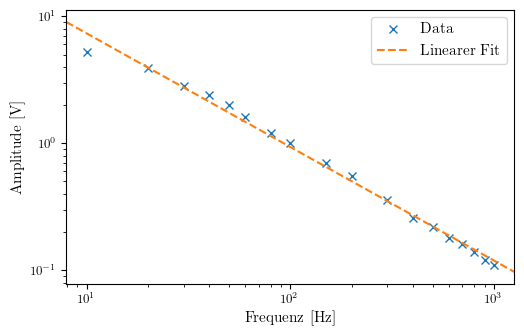
\includegraphics[width=0.6\textwidth]{Integrator}
\caption{Amplitude in Abhängigkeit von der Frequenz in doppellogarithmischer Darstellung für einen Integrator mit Widerstand $R=\SI{10}{\kilo\ohm}$ und Kapazität $C=\SI{100}{\nano\farad}$}
\label{fig:int}
\end{figure}

\begin{figure}
\centering
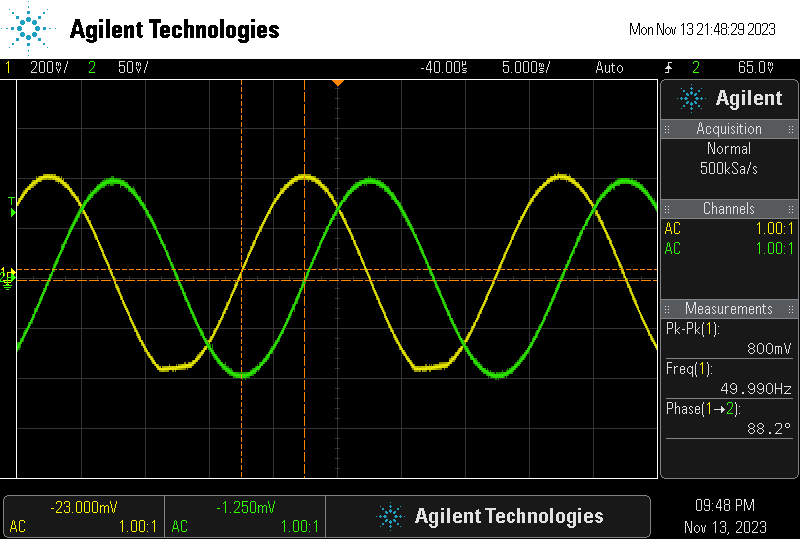
\includegraphics[width=0.6\textwidth]{scope_3}
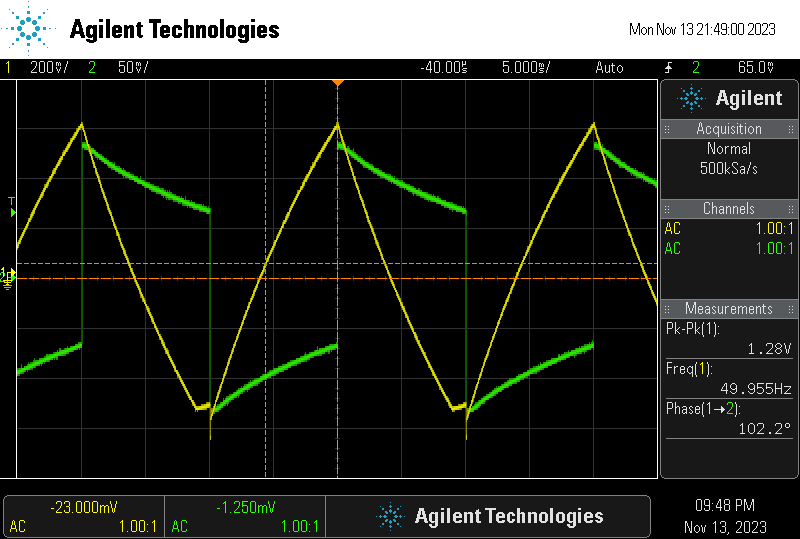
\includegraphics[width=0.6\textwidth]{scope_4}
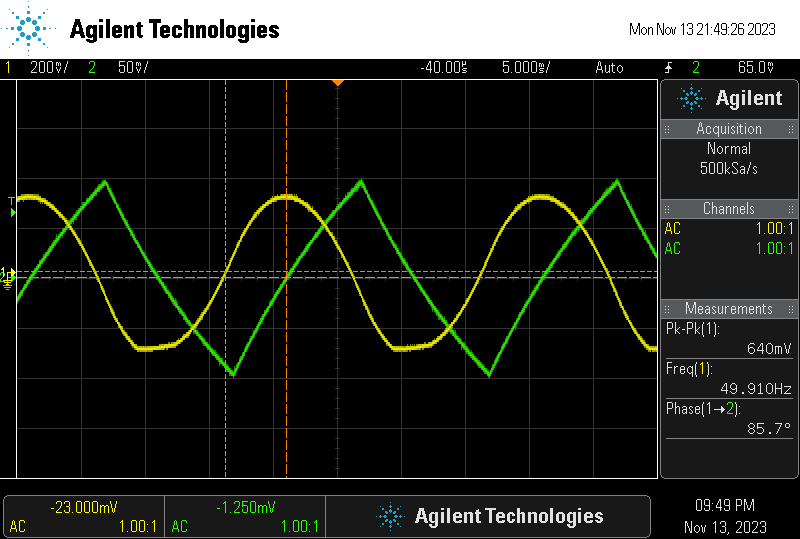
\includegraphics[width=0.6\textwidth]{scope_5}
\caption{Ausgangssignal eines Integrators (gelb) für eine Sinus-, Rechtecks- und Dreicksspannung als Eingangssignal (grün)}
\label{fig:int_screenshots}
\end{figure}
Abbildung $\ref{fig:int}$ zeigt die Amplitude der Ausgangsspannung in Abhängigkeit von der Frequenz. Zusätzlich ist eine Fitfunktion:
\begin{equation}
U_{int}(f)=(57,52\pm5,7)f^{-0,89\pm0,19}
\end{equation}
angelegt. Ein solcher Verlauf entspricht der Erwartung für den Verstärkungsverlauf eines Integrators.
Die Bilder in Abbildung $\ref{fig:int_screenshots}$ zeigen das Ausgangssignal des Integrators für verschiedene Eingangsspannungen. Wie zu erwarten ergibt sich aus einem Sinussignal nach Integration ein Kosinussignal, aus einer Rechteckspannung eine Dreieckspannung und aus einer Dreiecksspannung ein parabolischer Verlauf.
\subsection{Differentiator}
Der Differentiator verwendet einen Widerstand von $R=\SI{100}{\kilo\ohm}$ und eine Kapazität von $C=\SI{22}{\nano\farad}$.
\begin{figure}
\centering
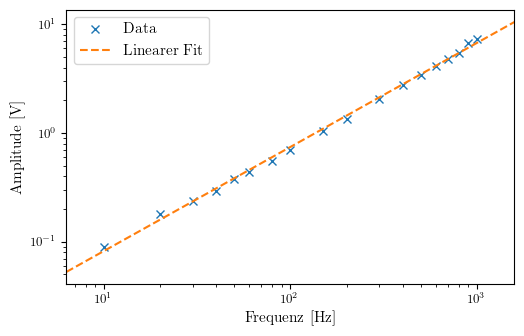
\includegraphics[width=0.6\textwidth]{Differentiator}
\caption{Amplitude in Abhängigkeit von der Frequenz in doppellogarithmischer Darstellung für einen Differentiator mit Widerstand $R=\SI{100}{\kilo\ohm}$ und Kapazität $C=\SI{22}{\nano\farad}$}
\label{fig:diff}
\end{figure}
\begin{figure}
\centering
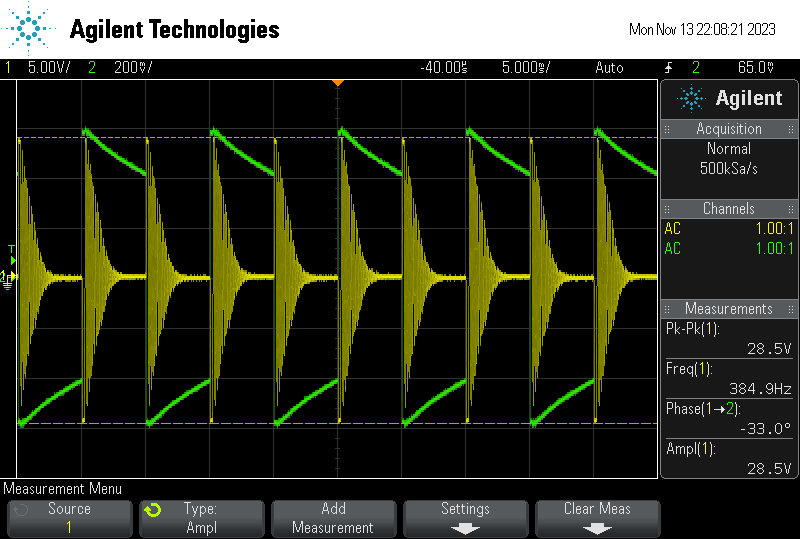
\includegraphics[width=0.6\textwidth]{scope_6}
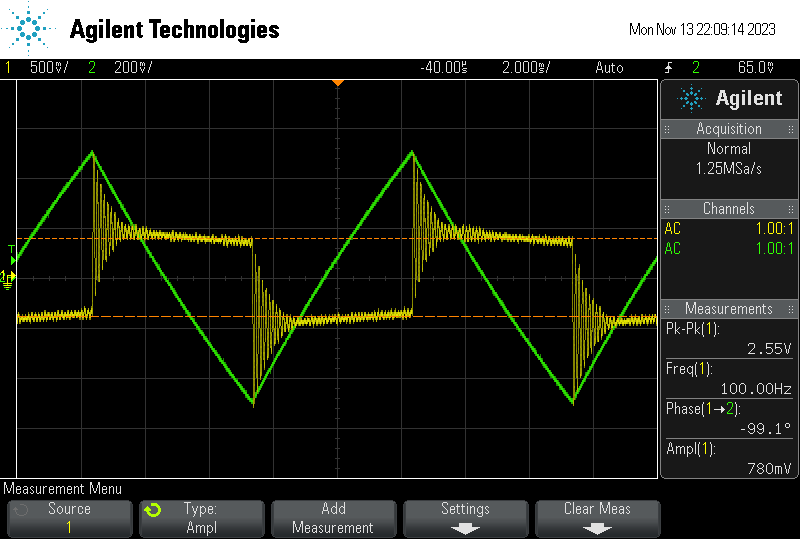
\includegraphics[width=0.6\textwidth]{scope_9}
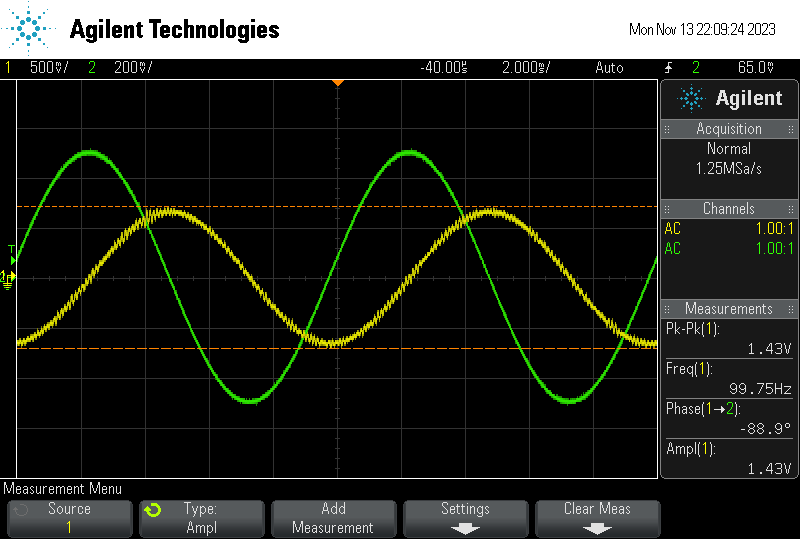
\includegraphics[width=0.6\textwidth]{scope_10}
\caption{Ausgangssignal eines Differentiators (gelb) für eine Sinus-, Rechtecks- und Dreicksspannung als Eingangssignal (grün)}
\label{fig:diff_screenshots}
\end{figure}
Die Amplitude des Ausgangssignals in Abhängigkeit von der Frequenz findet sich in Abbildung $\ref{fig:diff}$. Der zugehörige Fit lautet:
\begin{equation}
U_{diff}(f)=(0,009\pm0.000,5)f^{0,96\pm0,01}
\end{equation}
Wie zu erwarten steigt die Amplitude bzw. die Verstärkung mit steigender Frequenz an, wie sich auch im Fit zeigt.
Wie beim Integrator wird auch beim Differentiator durch die Fotos ($\ref{fig:diff_screenshots}$) die Reaktion auf die unterschiedlichen Eingangssignale veranschaulicht. Das Ausgangssignal erwartungsgemäß die Ableitung der jeweilligen Eingangsfunktion.
\subsection{Schmitt Triger}
Für den Schmitt Triger wurden die Widerstände $R_1=\SI{10}{\kilo\ohm}$ und $R_2=\SI{100}{\kilo\ohm}$ sowie die Betriebsspannungen $U_{\pm}=\pm\SI{15}{\volt}$ verwendet.
Somit ergeben sich die theoretischen Kippspannungen zu:
\begin{equation}
U_{kipp,\pm}=U_{\pm}\frac{R_1}{R_2}=\pm\SI{1,5}{\volt}
\end{equation}
Durch variiren der Amplitude des Eingangssignals konnte der Kippunkt und somit der Betrag der Kippspannung zu $U_{kipp}=\SI{1,465}{\volt}$ ermittelt werden. Weiterhin wurden durch Anlegen einer Dreieckspannung an jeweils drei Punkten der Kippunkt der Ausgangsspannung am Oszilloskop beobachtet. Durch Bildung der Mittelwerte führt dies zu den Kippspannungen:
\begin{gather}
U_{kipp,+}=\SI{1,567\pm0,06}{\volt} \\
U_{kipp,-}=\SI{1,5\pm0,058}{\volt}
\end{gather}
\subsection{Generator}
Für die Konstruktion des Generators wurden die Widerstände $R_1=\SI{10}{\kilo\ohm}$, $R_2=\SI{100}{\kilo\ohm}$ und $R_3=\SI{1}{\kilo\ohm}$ sowie die Kapazität $C=\SI{e-6}{\farad}$ verwendet. Dies liefert eine theoretische Frequenz des Ausgangssignals von:
\begin{equation}
f_a=\frac{R_2}{4CR_1R_3}=\SI{2,5}{\kilo\hertz}
\end{equation}
sowie eine Amplitude von
\begin{equation}
U_a=U_{max}\frac{R_1}{R_2}=\SI{1,4}{\volt}
\end{equation}
\begin{figure}
\centering
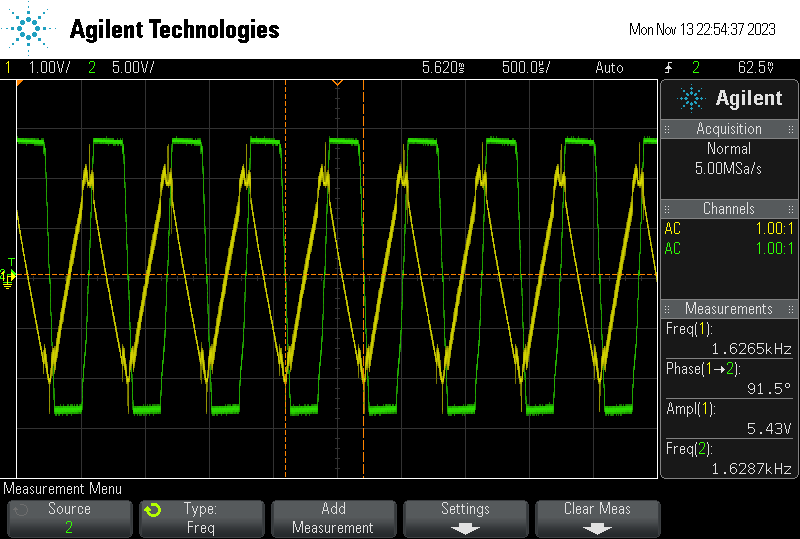
\includegraphics[width=0.6\textwidth]{scope_14}
\caption{Dreiecksschwingung und Rechteckschwingung des Generators}
\label{fig:Gen_screenshots}
\end{figure}
Die experimentellen Werte der generierten Ausgangsspannung $f_{a,exp}=\SI{1,62}{\kilo\hertz}$, $U_{a,exp}=\SI{2,1}{\volt}$ lassen sich der Abbildung $\ref{fig:Gen_screenshots}$ entnehmen. 
\subsection{Gedämpfte Schwingung}
Für die gedämpfte Schaltung wurde eine Schaltung mit den Kenndaten $R=\SI{1}{\kilo\ohm}$ und $C=\SI{100}{\nano\farad}$ verwendet.
\begin{figure}
\centering
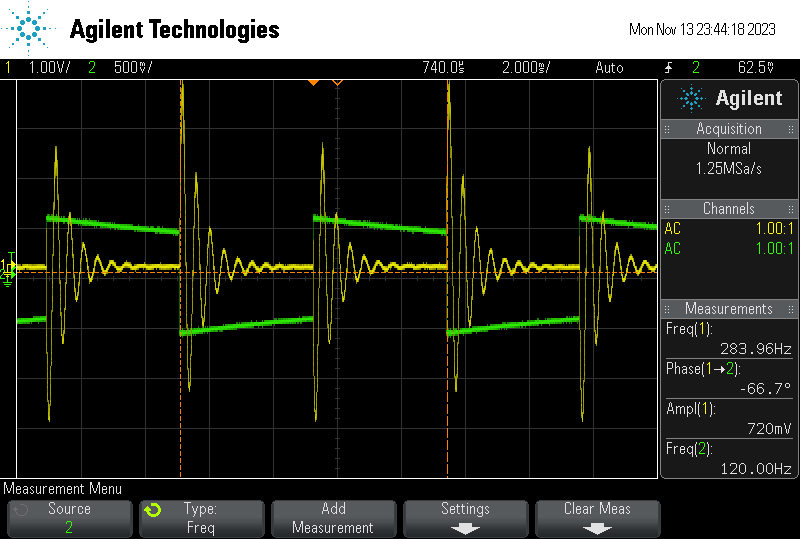
\includegraphics[width=0.6\textwidth]{scope_15}
\caption{Ausgangssignal eines Integrators (gelb) für eines- Sinus-, Rechteck und Dreicksspannung als Eingangssignal (grün)}
\label{fig:ged_screenshots}
\end{figure}
Die resultierende gedämpfte Schwingung ist in Abbildung $\ref{fig:ged_screenshots}$ zu sehen. Die theoretische Periodendauer lässt sich damit durch die Formel
\begin{equation}
T_{theo}=2\pi RC=\SI{628,3}{\micro\second}
\end{equation}
berechnen. Um die Periodendauer sowie die Abklingzeit $\tau$ zu berechnen wird eine der Schwingungen ausgewählt und ein exponentieller Fit an die Maxima angelegt um die Einhüllende zu bestimmen.
\begin{figure}
\centering
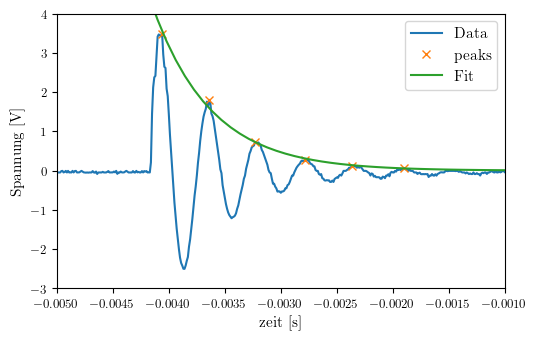
\includegraphics[width=0.49\textwidth]{ged schwing}
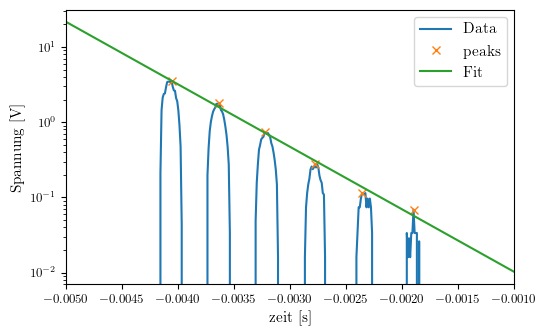
\includegraphics[width=0.49\textwidth]{ged schwing log}
\caption{Amplitude in Abhängigkeit von der Zeit für eine gedämpfte Schwingung in inearer und halblogarithmischer Darstellung}
\label{fig:ged_schwing}
\end{figure}
Das Ergebnis findet sich in Abbildung $\ref{fig:ged_schwing}$. Die zugehörige Fitfunktion lautet:
\begin{equation}
U_{schwing}(t)=a\exp(-mt)=(0,015\pm0,0004)\exp(-(1912,84\pm86,98)t)
\end{equation}
woraus die Abklingzeit
\begin{equation}
\tau=1/m=\SI{523\pm23,8}{\micro\second}
\end{equation}
bestimmt werden kann. Weiterhin kann durch die mittlere Distanz zwischen den Maxima die Periodendauer bestimmt werden:
\begin{equation}
T_{exp}=\SI{432\pm9,7}{\micro\second}
\end{equation}
